\documentclass[12pt]{article}[margin=1in]
\usepackage{fullpage,graphicx,psfrag,amsmath,amsfonts,verbatim}
\usepackage{multicol,multirow}
\usepackage[small,bf]{caption}
\usepackage{amsthm}
\usepackage{hyperref}
\usepackage{bbm} % for the indicator function to look good
\usepackage{color}
\usepackage{mathtools}
\usepackage{fancyhdr} % for the header
\usepackage{booktabs} % for regression table display (toprule, midrule, bottomrule)
\usepackage{adjustbox} % for regression table display
\usepackage{threeparttable} % to use table notes
\usepackage{natbib} % for bibliography
% \renewcommand{\familydefault}{\sfdefault}
\newcommand{\indep}{\perp\!\!\!\!\perp} % the independent symbol

% define theorem
\newtheorem{theorem}{Theorem}[section]
\newtheorem{corollary}[theorem]{Corollary}
\newtheorem{assumption}{Assumption}[subsection]
% define definition style
\theoremstyle{definition}
\newtheorem{definition}{Definition}[section]
\newtheorem{proposition}{Proposition}[section]
\newtheorem{property}{Property}[section]
\newtheorem{example}{Example}[section]
\newtheorem*{exercise}{Exercise}
% define remark style
\theoremstyle{remark}
\newtheorem*{remark}{Remark}
\newtheorem{question}{Question}

\newcommand{\R}{\mathbb{R}}
\newcommand{\C}{\mathbb{C}}
\newcommand{\Rd}{\mathbb{R}^d}
\newcommand{\Hy}{\mathbb{H}}
\newcommand{\calh}{\mathcal{H}}
\newcommand{\cala}{\mathcal{A}}
\newcommand{\calm}{\mathcal{M}}
\newcommand{\cald}{\mathcal{D}}
\newcommand{\caln}{\mathcal{N}}
\newcommand{\calr}{\mathcal{R}}
\newcommand{\calz}{\mathcal{Z}}
\newcommand{\caly}{\mathcal{Y}}
\newcommand{\calq}{\mathcal{Q}}
\newcommand{\cale}{\mathcal{E}}
\newcommand{\cali}{\mathcal{I}}
\newcommand{\calb}{\mathcal{B}}
\newcommand{\calc}{\mathcal{C}}
\newcommand{\calw}{\mathcal{W}}
\newcommand{\calg}{\mathcal{G}}
\newcommand{\calu}{\mathcal{U}}
\newcommand{\calo}{\mathcal{O}}
\newcommand{\calp}{\mathcal{P}}
\newcommand{\vect}{\mathrm{vect}}
\newcommand{\cov}{\mathrm{cov}}
\newcommand{\reff}{\mathrm{ref}}

\newcommand{\setbra}[1]{\left\{#1\right\}}
\newcommand{\set}[1]{\setbra{#1}}
\newcommand{\bra}[1]{\left[#1\right]}
\newcommand{\pa}[1]{\left(#1\right)}
\newcommand{\abs}[1]{\left| #1\right|}
\newcommand{\norm}[1]{\left\| #1 \right\|}
\newcommand{\angs}[1]{\left\langle #1\right\rangle}
\newcommand{\midvert}{\middle|}

\newcommand{\Q}{\mathbb{Q}}
\newcommand{\Lip}{\mathrm{Lip}}
\newcommand{\Z}{\mathbb{Z}}
\newcommand{\N}{\mathbb{N}}
\newcommand{\Cpx}{\mathbb{C}}
\newcommand{\E}{\mathbb{E}}
\newcommand{\V}{\mathbb{V}}
\newcommand{\Var}{\mathrm{Var}}
\newcommand{\p}{\mathbb{P}}
\newcommand{\F}{\mathcal{F}}
%\newcommand{\G}{\mathcal{G}}
\newcommand{\diag}{\mathrm{diag}}
\newcommand{\id}{\mathrm{id}}
\newcommand{\one}{\mathbbm{1}}
\newcommand{\defeq}{\overset{\mathrm{def}}{=}}
\newcommand{\nlr}{\nleftrightarrow}
\newcommand{\lr}{\leftrightarrow}
\newcommand{\ra}{\rightarrow}
\newcommand{\tr}{\mathrm{tr}}
\newcommand{\pspace}{(\Omega, \F, \p)}
\newcommand{\filt}{\pa{\F_t}_{0\leq t\leq \infty}}
\newcommand{\filtnat}{\pa{\F_t^X}_{0\leq t\leq \infty}}
\newcommand{\filtspace}{\pa{\Omega, \F, \filt, \p}}
\newcommand{\indist}[1]{\overset{d}{#1}}
\newcommand{\inlo}[1]{\overset{L^1}{#1}}
\newcommand{\inltwo}[1]{\overset{L^2}{#1}}
\newcommand{\inp}[1]{\overset{\p}{#1}}
\newcommand{\inpc}{\overset{\p}{\rightarrow}}
\newcommand{\indistc}{\indist{\rightarrow}}
\newcommand{\inas}[1]{\overset{\mathrm{a.s.}}{#1}}
\newcommand{\inhy}[1]{\overset{\mathrm{\Hy^2}}{#1}}
\newcommand{\cc}[1]{\mathrm{CC}\left(#1 \right)}
\newcommand{\partfrac}[1]{\frac{\partial}{\partial #1}} \newcommand{\Chi}{\mathcal{X}} \newcommand{\tl}{{T,\Lambda}}
\newcommand{\isingspace}{\{\pm\}^\Lambda} \newcommand{\boltzmeas}{\mu_\tl}
\newcommand{\bl}{{\beta, \Lambda}} \newcommand{\zerot}{{t\in [0,T]}}
\newcommand{\tgez}{{t\geq 0}} \newcommand{\brown}{(B_t)_\tgez}
\newcommand{\process}{(X_t)_\tgez} \newcommand{\smallising}[4]{\begin{matrix} #1&#2\\#3&#4\end{matrix}}
\def\ci{\perp\!\!\!\!\perp}
\newcommand{\parm}{{(m)}} \newcommand{\diff}{\mathrm{d}} \newcommand{\optp}{\mathrm{opt}_\p}
\newcommand{\erp}{\mathrm{er}_\p} \newcommand{\er}{\mathrm{er}}
\newcommand{\sgn}{\mathrm{sgn}} \DeclareMathOperator*{\argmin}{arg\,min}
\DeclareMathOperator*{\argmax}{arg\,max}
\DeclareMathOperator*{\esssup}{ess\,sup}
\DeclareMathOperator*{\essinf}{ess\,inf} \newcommand{\vcdim}{\mathrm{VCdim}}
\newcommand{\bigargs}{\pa{\bar{Y}_t,M_t,\theta_t}}
\newcommand{\bigargsm}{\pa{\bar{Y}_{t-},M_{t-},\theta_{t-}}}
\newcommand{\smallargs}{\pa{\bar{y},m,\vartheta}}
\newcommand{\smallarg}{\pa{m,\vartheta}}

\newcommand{\fatone}{\mathbf{1}}
\newcommand{\pen}{\mathrm{pen}}
\newcommand{\MF}{\mathrm{MF}}
\newcommand{\opt}{\mathrm{opt}}
\newcommand{\MSE}{\mathrm{MSE}}
\newcommand{\MISE}{\mathrm{MISE}}
\newcommand{\CV}{\mathrm{CV}}

\newcommand{\1}{\mathbbm{1}}
\newenvironment{sol}{\begin{proof}[Solution]}{\end{proof}}


\bibliographystyle{apalike}
\setlength{\parindent}{0pt} % remove the automatic indentation % for problem set
\renewcommand{\thesection}{Section \arabic{section}}
\renewcommand{\thesubsection}{\arabic{section}.\arabic{subsection}}

% Settings for page number in the footer
\pagestyle{fancy}
\fancyhf{}
\fancyfoot[C]{\thepage}
\renewcommand{\headrulewidth}{0pt}
\renewcommand{\footrulewidth}{0pt}

\title{\textbf{Linear Regression Equation from DDC} \\
\vspace{.3cm}
\large Coding Exercise \\
Environmental Economics}
\author{Zixuan}
\date{\today}

\begin{document}
\maketitle

\section{Spatial Data}

\begin{enumerate}
    \item Reclassify crops based on land use and irrigation.
    \item Calculate the size of grids.
    \item Show the distribution of irrigated and non-irrigated croplands in Almeria in 2021 ~\ref{fig:land_use_distribution_almeria_2021}.
    \item Irrigated area by crop and aggregate over time ~\ref{fig:irrigated_area_by_crop_over_time}.
    \item Average area by crop ~\ref{tab:area_by_crop_avg}. Average area by crop and irrigation ~\ref{tab:area_by_crop_irr_avg}.
\end{enumerate}


\begin{figure}[!htbp]
    \centering
    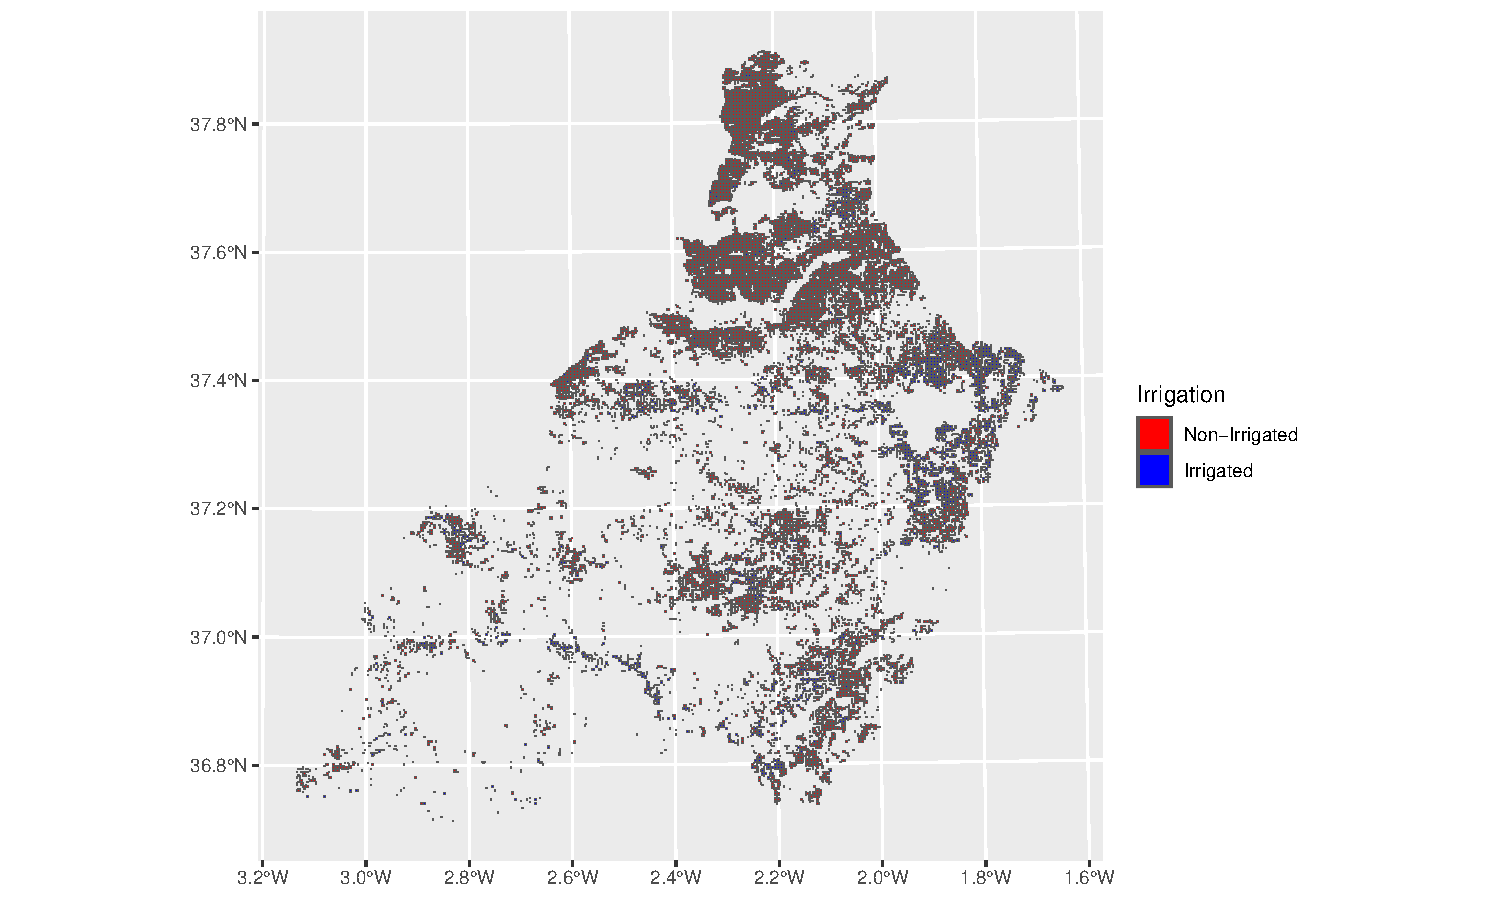
\includegraphics[width=0.8\textwidth]{../Figures/land_use_distribution_almeria_2021.pdf}
    \caption{Distribution of irrigated and non-irrigated croplands in Almeria in 2021.}
    \label{fig:land_use_distribution_almeria_2021}
\end{figure}

\begin{figure}[!htbp]
    \centering
    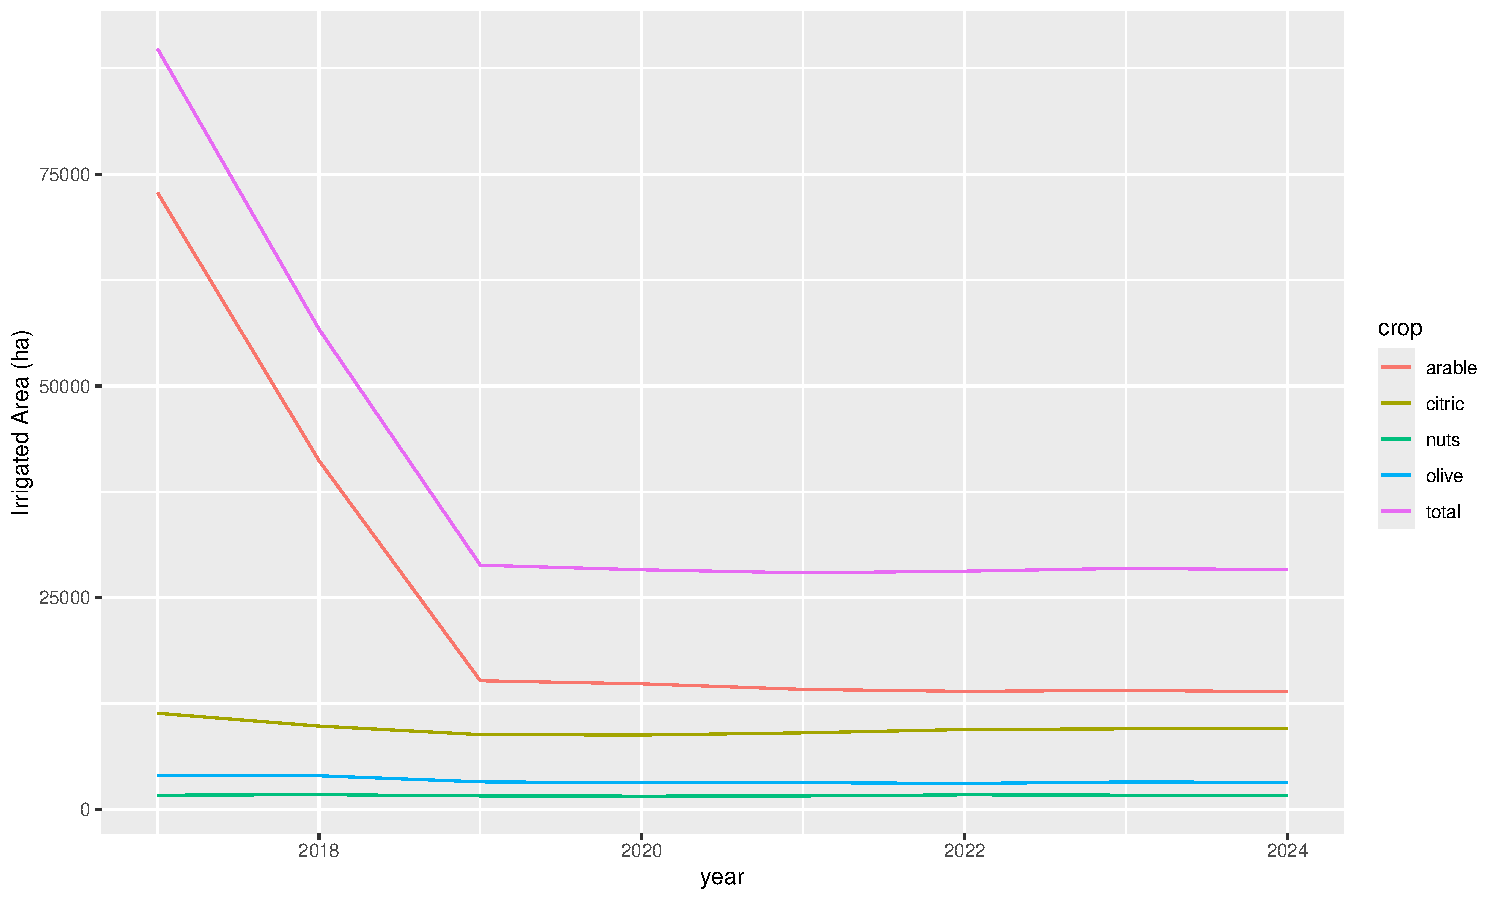
\includegraphics[width=0.6\textwidth]{../Figures/irrigated_area_by_crop_over_time.pdf}
    \caption{Irrigated area by crop and aggregate over time.}
    \label{fig:irrigated_area_by_crop_over_time}
\end{figure}

\begin{table}
    \centering
    % latex table generated in R 4.4.2 by xtable 1.8-4 package
% Fri Jun 20 10:22:01 2025

\begin{tabular}{lr}
  \hline
  crop   & avg\_area\_ha \\
  \hline
  arable & 149535.16     \\
  olive  & 9780.47       \\
  nuts   & 59607.03      \\
  citric & 9535.94       \\
  \hline
\end{tabular}


    \caption{Average area by crop.}
    \label{tab:area_by_crop_avg}
\end{table}

\begin{table}
    \centering
    % latex table generated in R 4.4.2 by xtable 1.8-4 package
% Fri Jun 20 10:22:49 2025
\begin{table}[ht]
\centering
\begin{tabular}{lrr}
  \hline
crop & irrigation & avg\_area\_ha \\ 
  \hline
arable &   0 & 124530.47 \\ 
  olive &   1 & 3368.75 \\ 
  arable &   1 & 25004.69 \\ 
  olive &   0 & 6411.72 \\ 
  nuts &   0 & 57960.16 \\ 
  nuts &   1 & 1646.87 \\ 
  citric &   1 & 9535.94 \\ 
   \hline
\end{tabular}
\end{table}

    \caption{Average area by crop and irrigation.}
    \label{tab:area_by_crop_irr_avg}
\end{table}


\section{Model}
Instead of directly answering the questions, I develop the estimating equation in the following way (which answers the question indirectly).

\paragraph{State} Usually, we write the observed state as $s$ and unobserved state as $\varepsilon$.

Here, the observed state has to two components: the individual state $k$ and the aggregate state $\omega$. 
\begin{enumerate}
    \item $k$ evolves deterministically, i.e. $k_{t+1} = a_t$
    \item $\omega$ evolves in the following way, $G(\omega_{t+1} | \omega_t, a_t) = G(\omega_{t+1} | \omega_t)$
\end{enumerate}

\paragraph{Reward function and Value function}

I denote the reward function as $u(k, \omega)$, and the continuation reward function as $\tilde{u}(k, \omega,a) = u(k, \omega, a) + \beta \E\bra{\tilde{V}_{t+1}(k_{t+1}, \omega_{t+1}) | k, \omega, a}$.

Also  value function is written as $V_t(k,\omega, \varepsilon)$ and the expected value function $\bar{V}_t(k,\omega)$. 

\paragraph{Derivation} There is a nice relationship between the expected value function and the continuation reward function, which is
$$ \bar{V}_t(k, \omega) = \tilde{u}(k, \omega, a) + \psi_a(p(k,\omega))$$  for any choice of action $a$.
In the form that we are more familiar with by imposing the standard assumption on $\varepsilon$,
$$ \bar{V}_t(k, \omega) = \tilde{u}(k, \omega, a) + \gamma -\Pr(a_t = a | k, \omega) $$

Now let us take another chioce $a_t=j$ which gives exactly the same stuff
$$ \bar{V}_t(k, \omega) = \tilde{u}(k, \omega, a) + \psi_a(p(k,\omega)) $$
Then we can take the difference between the two equations above,
$$ \psi_j(p(k,\omega)) - \psi_a(p(k,\omega)) = \tilde{u}(k, \omega, a) - \tilde{u}(k, \omega, j) $$
Imposing the standard assumption on $\varepsilon$ such that $\psi_a(p(k,\omega)) = \gamma - \log \Pr(a_t = a | k, \omega)$.
The left hand side becomes $$ \log \frac{\Pr(a_t = j | k, \omega)}{\Pr(a_t = a | k, \omega)} $$
Look at the right hand side, how to express the $\tilde{u}(k, \omega, a)$ as an explicit function of observed variables and parameters? 
First, recall that individual state $k$ evolves deterministically,
$$ \tilde{u}(k, \omega, a)  = u(k, \omega, a) + \beta \E\bra{\bar{V}_{t+1}(a, \omega_{t+1}) | k, \omega, a} $$
Then how to make use of renewal action? For example, we choose $a_t = a$ and $a_{t+1} = r$ OR $a_t = j$ and $a_{t+1} = r$. Since we the individual state is equal to the last period action, even if we are not switching crop, as long as we choose the same action, the individual state is the same (one period finite dependence?)
$$ \E_{\omega_{t+1}|j,\omega} \bar{V}_{t+1}(r, \omega_{t+1}| j, \omega, r) = \E_{\omega_{t+1}|a,\omega}\bar{V}_{t+1}(r, \omega_{t+1}| a,\omega, r)$$

Recall in the case of \citet{scott2014dynamic}, the renewal action is choosing crop, the state $k$ is the number of years up to now that the land is not used for growing crops. 
$$ \E_{\omega_{t+1}} \bar{V}_{t+1}(k_{t+1}=2, \omega_{t+1}|k=1,\omega, a=\text{other}) \neq \E_{\omega_{t+1}} \bar{V}_{t+1}(k_{t+1}=3, \omega_{t+1}| k=2,\omega, a=\text{other})$$
But 
$$ \E_{\omega_{t+1}} \bar{V}_{t+1}(k_{t+1}=0, \omega_{t+1}|k=1,\omega, a=\text{crop}) = \E_{\omega_{t+1}} \bar{V}_{t+1}(k_{t+1}=0, \omega_{t+1}| k=2,\omega, a=\text{crop})$$

Back to the problem set, we have that by 
$$ \tilde{u}_t(k, \omega, a) = u_t(k, \omega, a) + \beta \E_{\omega_{t+1}} \bar{V}_{t+1}(a, \omega_{t+1}| k, \omega, a) $$
Similarly for $\tilde{u}_t(k, \omega, j)$, but of course 
$$ \E_{\omega_{t+1}|\omega} \bar{V}_{t+1}(a, \omega_{t+1}| k, \omega, a) \neq \E_{\omega_{t+1}|\omega} \bar{V}_{t+1}(j, \omega_{t+1}| k, \omega, j) $$ But if we look one period ahead, choosing the same action at $t+1$, then 
$$ \E_{\omega_{t+2}|\omega'}\bar{V}_{t+2}(r, \omega_{t+2}| a, \omega', r) = \bar{V}_{t+2|\omega'}(r, \omega_{t+2}| j, \omega', r) $$
Then the right hand side becomes
\begin{equation}
    \begin{split}
        \tilde{u}_t(k, \omega, a) - \tilde{u}_t(k, \omega, j) & = u_t(k, \omega, a) - u_t(k, \omega, j)                                                                                                                                                 \\
                                                              & + \beta\E_{\omega_{t+1}|\omega} \bra{u_{t+1}(a, \omega_{t+1},r) -\ln \Pr_{t+1}(r | a, \omega_{t+1}) + \E_{\omega_{t+2}|\omega_{t+1}}\bar{V}_{t+2}(r, \omega_{t+2}| a, \omega_{t+1}, r)} \\
                                                              & - \beta\E_{\omega_{t+1}|\omega} \bra{u_{t+1}(j, \omega_{t+1},r) -\ln \Pr_{t+1}(r| j, \omega_{t+1}) + \E_{\omega_{t+2}|\omega_{t+1}}\bar{V}_{t+2}(r, \omega_{t+2}| j, \omega_{t+1}, r)}  \\
                                                              & = u_t(k, \omega, a) - u_t(k, \omega, j) + \beta \E_{\omega_{t+1}|\omega} \bra{u_{t+1}(a, \omega_{t+1},r) - u_{t+1}(j, \omega_{t+1},r)}                                                  \\
                                                              & + \beta \E_{\omega_{t+1}|\omega} \bra{\ln \Pr_{t+1}(r | a, \omega_{t+1}) - \ln \Pr_{t+1}(r | j, \omega_{t+1})}
    \end{split}
\end{equation}

Since we don't know the evolution fo aggregate state $\omega$ (we didn't even define it), by fixing one $\omega_{t+1}=\omega'$ and
\begin{equation}
    \begin{split}
        \tilde{u}_t(k, \omega, a) - \tilde{u}_t(k, \omega, j) & = u_t(k, \omega, a) - u_t(k, \omega, j)                                                                                                        \\
                                                              & + \beta\bra{u_{t+1}(a, \omega',r) -\ln \Pr_{t+1}(r | a, \omega') + \E_{\omega_{t+2}|\omega'}\bar{V}_{t+2}(r, \omega_{t+2}| a, \omega', r)  }   \\
                                                              & -\beta \bra{u_{t+1}(j, \omega',r) -\ln \Pr_{t+1}(r| j, \omega') + \E_{\omega_{t+2}|\omega_{t+1}}\bar{V}_{t+2}(r, \omega_{t+2}| j, \omega', r)} \\
                                                              & + e_t(\omega',\omega, a) -e_t(\omega',\omega, j) 
    \end{split}
\end{equation}
where $e_t(\omega',\omega, a) = \beta \E_{\omega_{t+1}|\omega} \bar{V}_{t+1}(a, \omega_{t+1}| k, \omega, a)  - \beta \bar{V}_{t+1}(a, \omega'| k, \omega, a)$ which is the difference between the expecatation over $\omega_{t+1}|\omega$ and a random fixed $\omega_{t+1}=\omega'$.

Therefore the regression equation is 
\begin{equation}
    \begin{split}
        \log \frac{\Pr(a_t = j | k, \omega)}{\Pr(a_t = a | k, \omega)} + \beta \log \frac{\Pr_{t+1}(r | a, \omega')}{\Pr_{t+1}(r | j, \omega')} & = u_t(k, \omega, a) - u_t(k, \omega, j) \\ &+ \beta\bra{u_{t+1}(a, \omega',r) - u_{t+1}(j, \omega',r)} + e_t(\omega',\omega, a) - e_t(\omega',\omega, j)
    \end{split}
\end{equation}

Plug in the functional form of the reward function,
$$ u_t(k, \omega=(m,\eta), a) = \theta_a+\theta_{ka}+\theta_R R(m,a) + \xi(k, \omega, a)$$
Then the regression equation is 
\begin{itemize}
    \item $ Y_{tk}  = \log \frac{\Pr(a_t = j | k, \omega)}{\Pr(a_t = a | k, \omega)} + \beta \log \frac{\Pr_{t+1}(r | a, \omega')}{\Pr_{t+1}(r | j, \omega')}$
    \item $\theta_j-\theta_a + \theta_{kj} - \theta_{ka} + \beta(\theta_{jr}-\theta_{ar})$
    \item $\theta_R(R(m,a) - R(m,j))$
    \item $\xi(k, \omega,j) - \xi(k, \omega,a) + \beta(\xi_{t+1}(j, \omega',r) - \xi_{t+1}(a, \omega',r))$
    \item $e_t(\omega',\omega, a) - e_t(\omega',\omega, j)$
\end{itemize}


This is like the when we use market share data to estimate the parameters. In a market,
$$ \log(s_j/s_0)=\alpha+ \beta X_j + \xi_j$$
With multiple years of observations of the market.
$$ \log(s_{jt}/s_{0t}) = \alpha + \beta X_{jt} + \xi_{jt}$$
if for a given $j$, $\xi_{jt}$ is correlated across time, we should control for it $\xi_{jt} = \xi_j + \varepsilon_{jt}$. 
Then use the fixed effect estimator etc. 
Similarly here, the unit of observation is $k-j-a-r$. and fixed effect corresponds to. 

\paragraph{Source of variation} The identifying variation is cross sectional variation in $R(m,j) - R(m,a)$ for different $j-a$ pairs and across time variation $R_t(m,j) - R_t(m,a)$ over different $t$ (becasue we need to take difference later!).

\paragraph{Endogeneity} First, ignoring the fixed effect term, he terms xxx in the euqation are treated as the error term in the regression but one needs to justify that
they are uncorrelated with $\Delta R(m,j,a)$ (across section endogeneity). For example, it may be the case the individual land $\xi(k, \omega, a)$ is uncorrelated with some variables $m$, and $R(m,j)$ is correlated with that $m$. Then we can use $m$ as the instrument. 

Secondly, to remove fixed effect, we need to take first difference, which introduces more endogeneity concerns (over time endogeneity). For example, the error term $\xi(k, \omega, a)$ is correlated with $R(m,j)$ over time. The first difference GMM estimator can be used to deal with the issue. Use lagged values of regressors $x_{t-2}$ as instruments for the first difference of the regressors $\Delta x_{t}=x_{t}-x_{t-1}$.


\paragraph{Restriction and normalization}
\begin{enumerate}
    \item How many fixed effect can we estimate? $|k|^4$ fixed effects.
    \item How many parameters do we have? $|k|+|k|^2$.
\end{enumerate}
If we just fix one $j-a-r$, there are $|k|$ fixed effect, and $2|k|+1$ parameters ($\theta_{kj}$,$\theta_{ka}$,the rest) to estimate. Some restrictions are needed. 


\begin{enumerate}
    \item we set $\theta_{ka}$ to be the same for all $k$. reduce by $|k|-1$.
    \item we assume non-switching cost is zero such that $\theta_{jj}=0$. reduce by 1.
    \item one more restriction is needed. therefore we set $\theta_{ka}=0$ as well. reduce by 1.
\end{enumerate}

But this is actually not necessary. Perhaps we have over identifification. But I will just leave it there as it is.




% Keeping the standard assumption on $\varepsilon$, the ccp takes the form of 
% $$ \Pr(a_t = a | k, \omega) = \frac{\exp \tilde{u}(k, \omega, a)}{\sum_{a' \in A} \exp \tilde{u}(k, \omega, a')} $$


\section{Estimation}

\paragraph{Observations filtering}
We restrict ourselves to the following two paths of actions, rather than any possible paths. 
\begin{enumerate}
    \item $k\to k\to a$
    \item $k\to a \to a$
\end{enumerate}

Therefore we have
\begin{itemize}
    \item $Y_{tk}  = \log \frac{\Pr(a_t = k | k, \omega)}{\Pr(a_t = a | k, \omega)} + \beta \log \frac{\Pr_{t+1}(a | k, \omega')}{\Pr_{t+1}(a | a, \omega')}$
    \item $\theta_k-\theta_a + \theta_{kk} - \theta_{ka} + \beta(\theta_{ka}-\theta_{aa})$
    \item $\theta_R(R(m,a) - R(m,k))$
    \item $\xi(k, \omega,k) - \xi(k, \omega,a) + \beta(\xi_{t+1}(k, \omega',a) - \xi_{t+1}(a, \omega',a))$
    \item $e_t(\omega',\omega, a) - e_t(\omega',\omega, k)$
\end{itemize}

\paragraph{Left-hand side variable}
To construct the left-hand side variable of the estimating equation, we need to estimate the choice probability first $\Pr(a_t = a | k, \omega)$.
For each province-year-state-action pair, we use the frequency of action as the probability.

\paragraph{Right-hand side variable}
To construct the right-hand side variables, we estiamte the return by first predicting the yields and price, then plus subsidies and minus costs. 
The estimating equation is that we split the data into subcrop category, then we run for each category

\verb| lm(log(yield) ~ DD30 * precipitation + DD10 * precipitation + year + prov )|

There seems to large differences between the predicted return and the actual return. Finer data maybe helpful as in \citet{scott2014dynamic} because in that paper, there are both state, country and land, three levels. While here we only have province and land. If there is a county level data on weather, we can better predict the return. 

In the following estimation, I used the actual return.

\paragraph{Panel data estimation}

We first take difference to remove the fixed effect. Then we use the lagged value $x_{k,t-2}$ as the instrument for the first difference of the regressors $\Delta x_{kt} = x_{kt} - x_{k,t-1}$.

The esimating moment condition is 
$$
    E[(\Delta y_{kt} - \beta \Delta x_{kt}) \cdot x_{k,t-2}] = 0
$$


\paragraph{Recover fixed effect and switching cost parameters}

We use the following equations to recover the fixed effect $\alpha_i$ where $\bar{y}_i,\bar{x}_i$ is the time average. And $i$ is the index for the unit (k-a pair)
$$
    \hat{\alpha}_i = \bar{y}_i - \beta \bar{x}_i
$$

Recall that

$$
    \alpha_{ka} = \theta_k-\theta_a + \theta_{kk} - \theta_{ka} + \beta(\theta_{ka}-\theta_{aa}) = \theta_k-\theta_a- \theta_{ka} + \beta \theta_{ka}$$


\begin{enumerate}
    \item step 1: pick any $k_1$ and $a_0 = \text{other}$, we have $\alpha_{k_1 a_0}-\alpha_{a_0 a_0} = \theta_{k_1} - \theta_{a_0} + (\beta-1)(\theta_{k_1 a_0} - \theta_{a_0 a_0}) = \theta_{k_1} - \theta_{a_0}$
    \item step 2: pick any $a_1$  Then $\alpha_{k_1 a_1}-\alpha_{k_1 a_0} = \theta_{a_0}- \theta_{a_1} + (\beta -1)(\theta_{k_1 a_1 }-\theta_{k_1 a_0}) = \theta_{a_0}- \theta_{a_1} + (\beta -1)\theta_{k_1 a_1 }$
          Since we can get any $\theta_{a_0}- \theta_{a_1}$ from step 1. Then we can automatically recover $\theta_{k_1a_1}$
    \item fixing $k_1$ and $a_1$ to be of the same crop but different irrigation will give irrigation switching cost. fixing them of differnt crops but same irrigation will give crop switching cost.
\end{enumerate}

\paragraph{Myopic and static model}
\begin{itemize}
    \item For the myopic model, we set $\beta=0$ and everthing else the same.
    \item For the static model which basically entirely removes state dependence. We need to recalculate the choice probability not conditional on state. T
          $$ \log(p_{jt}/p_{0t}) = \alpha + \beta X_{jt} + \xi_{jt} = \beta X_{jt}+\xi_j + \varepsilon_{jt}$$
          Then use the GMM as above. 
\end{itemize}


\bibliography{ref.bib}

\end{document}


